\chapter{Cosmic rays and the Pierre Auger Observatory}
\label{sec:uhecr}


\cite{Mollerach:2017idb}

%%%%%%%%%%%%%%%%%%%%%%%%%%%%%%%%%%%%
\section{Overview of cosmic rays}
\label{sec:uhecr:overview}

%%================================%%
\subsection{History}

-history: HESS, Auger and UHE

%%================================%%
\subsection{Energy spectrum}

%%%%%%%%%%%%%% SPEC SWORDY %%%%%%%%%%%%%%%
\begin{wrapfigure}{r}{0.55\textwidth}
  \centering
  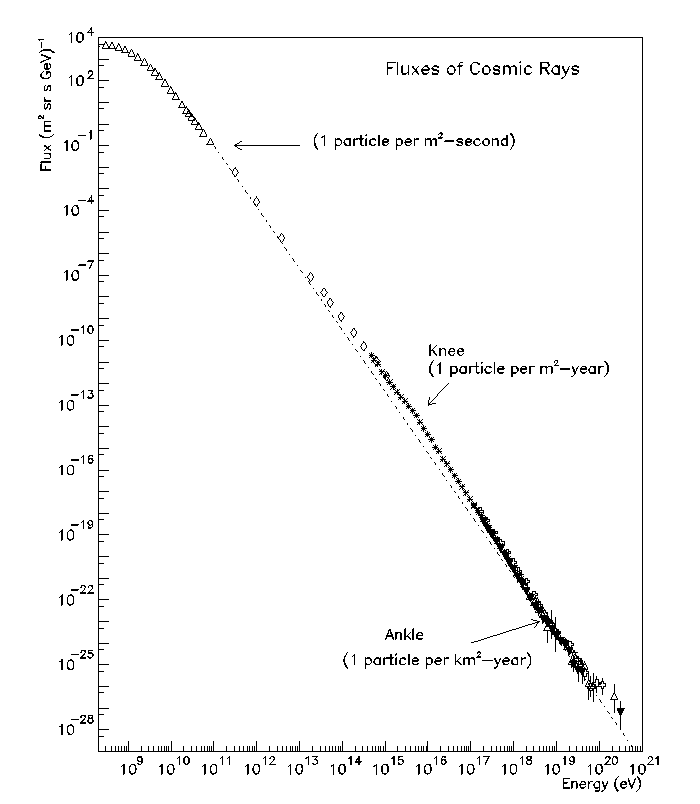
\includegraphics[width=0.55\textwidth]{spectrum_swordy}
  \caption{\cite{SwordyPlot2001}}
  \label{fig:uhecr:overview:spec:swordy}
\end{wrapfigure}

The cosmic rays flux as a function of its energy, the so called \emph{energy spectrum},
plays a central hole in the understanding of the astrophysical aspects behind these particles.
A compilation of measurements of the cosmic rays
energy spectrum over about 13 orders of magnitude
in energy is shown in~\cref{fig:uhecr:overview:spec:swordy}
One can see that from about \E{11} up to the highest energies
the spectrum can be described approximately 
by a power law $\text{d}\phi/\text{d}E \sim E^{-\gamma}$, where
the spectral index $\gamma$ is not exactly constant over all the energy range
but it changes only slightly between 2.5 and 3.2.
Because the cosmic rays spectrum extends over a very large
energy range, it is expected that different astrophysical mechanisms,
occuring at distinct scales, contribute to the origin
of the cosmic rays from different regions of the spectrum. As an illustration
we can point out that most of the modern models assume that the cosmic rays flux
is dominated by particles produced inside our galaxy up to around \e{17}-\E{18} and
an extragalactic origin for particles above this energy. The transition between
these two components is currently one of the most relevant topics of discussion.


Because of the spectrum steepness, the particle fluxes change over 27 orders of magnitude
from \e{11} and \E{21}. As indicated in~\cref{fig:uhecr:overview:spec:swordy},
while at \E{11} the flux is about 1 particle/m$^2$/second,
at \E{19} it drops to only 1 particle/km$^2$/year.
As a consequence, different experimental techniques have to be used to detect
cosmic ray particles at different energy ranges. Up to around \E{14}, the low flux
allows us to use small area instruments installed in ballons or satellites
to detects the particles before they interact with the earth's atmosphere.
Above this energy, the interaction with the atmosphere turns to be
useful since we can measure the cosmic rays indirectly through the detection of
the extensive air showers (see~\cref{sec:showers}). For that, large arrays of detectors
are used and their areas can vary substantially depending on the energy range they are
intended to study. As an example, the KASCADE experiment~\cite{\KASCADEPaper}
that is designed to measure particles from around \e{14} to \E{16}
has an area of 4000 m$^2$, while Pierre Auger
Observatory~\cite{\AugerPaper} has an area of 3000 km$^2$ to measure particles above \E{18}.

%%================================%%
\subsubsection{Main features of the energy spectrum}

The features of the cosmic ray spectrum are identified by the changes on the
spectral index $\gamma$. To better visualize these changes, we show
in~\cref{fig:uhecr:overview:spec:pdg} a compilation of measurements of
the spectrum from \E{13} in which the flux is scaled by a factor $E^{2.6}$.
As indicated in~\cref{fig:uhecr:overview:spec:pdg}, the first feature
is the so called \emph{first-knee} and it occurs around $3\times\E{15}$. At this energy
the index changes from $\gamma\approx 2.7$ to $3.0$. The next feature is
the \emph{second-knee}, around \E{17}, where there is a further steepening
and the index goes to $\gamma\approx 3.3$. The spectrum then becomes harder again
at the \emph{ankle}, around $5\times\E{18}$, where the index changes to $\gamma\approx 2.6$.
The final feature occurs at the highest energies, above $4\E{19}$, where the
value of the spectral index becomes very high ($>4$), caracterizing the so called
\emph{suppression}.


%%%%%%%%%%%%%% SPEC PDG %%%%%%%%%%%%%%%
\begin{figure}
  \centering
  
  \begin{overpic}[clip, rviewport=0 0 1 1,width=0.8\textwidth]{spectrum_pdg}
    \put(18,60){}
  \end{overpic}
  
  \caption{\cite{\PDGPaper}.}
  \label{fig:uhecr:overview:spec:pdg}
\end{figure}

The consistent interpretation of all these spectrum features requires the knowledge
about the composition of the cosmic rays. Particularly in the energy region compreending
the first and second-knee, very efficient composition measurements were performed
by KASCADE~\cite{\KASCADEPaper} and
KASCADE-Grande~\cite{\KASCADEGrandePaper} experiments. By using an experimental setup
that included surface detectors able to measured both number of charged particles and
number of muons in air showers, it was possible to measure the all particle spectrum
as well as to infer the spectra of individual groups of particles. In~\cref{}
we show the results of both experiments. Althought the final spectra are
strongly dependend on the hadronic interaction models
(see~\cref{sec:shower:simulations:models}) used in the analysis,
it is still possible to conclude that: (a) the first-knee is the result
of the suppression of the proton component of the spectrum~\cite{Antoni:2005wq},
(b) the suppression of the heavier components is consistent with
a rigidity dependent suppression~\cite{Antoni:2005wq} and (c) the second-knee coincides
with the suppression of the heaviest group of particles,
including iron nuclei~\cite{Apel:2011mi,Apel:2013uni}. 

Although the rigidity dependent suppression as an explanation for the knee
was a known hypothesis since it was suggested by Peters, in 1961~\cite{Peters1961},
the actual explanation is still a matter of discussion. The most simple
model would assume that the suppression is a consequence of a limit
in the maximum energy reachable by the sources~\cite{Gaisser:2013bla}.  
Alternative models include explanations based on the effect of the
drifting of cosmic rays in the galactic magnetic field~\cite{Ptuskin1993,Candia:2002qd}
and on the escape of cosmic rays from the galaxy~\cite{Giacinti:2014xya}.
Most of the models, however, converge on the fact that up to the second-knee
the cosmic ray flux is dominated by a galactic component. The transition
between this galactic and an extra-galactic component would then occur
at energies around the second-knee and the ankle.
The measurements and the models concerning this energy range (above \E{17}),
which is the range of interest of this thesis,
will be presented in~\cref{sec:uhecr:spectrum}.


%%================================%%
\subsection{Acceleration and sources}



%%================================%%
\subsection{Propagation}


-spectrum: knee, 2nd knee, ankle and GZK

-further: arrival directions, propagation, gamma/neutrinos, ...

-Fermi, 1st and 2nd order

-Hillas plot

-

%%%%%%%%%%%%%%%%%%%%%%%%%%%%%%%%%%%%
\section{Energy spectrum and composition at ultra-high energies}
\label{sec:uhecr:spectrum}

-hypothesis for ankle and GZK

-combined fit

-composition at the highest energies


%%%%%%%%%%%%%%%%%%%%%%%%%%%%%%%%%%%%
\section{The Pierre Auger Observatory}
\label{sec:uhecr:auger}


%%================================%%
\subsection{AugerPrime}






